\documentclass[12pt]{article}

%packages
%\usepackage{latexsym}
\usepackage{graphicx}
\usepackage{wrapfig}
\usepackage{color}
\usepackage{amsmath}
\usepackage{dsfont}
\usepackage{placeins}
\usepackage{amssymb}
\usepackage{skull}
\usepackage{enumerate}
\usepackage{soul}
\usepackage{alphalph}
\usepackage{hyperref}
\usepackage{enumerate}
\usepackage{listings}
\usepackage{multicol}
\usepackage{etoolbox}
%\usepackage{fancyhdr}

%\fancyhf{} % clear all header and footers
%\renewcommand{\headrulewidth}{0pt} % remove the header rule
%\fancyfoot[LE, LO]{\thepage}


%\usepackage{pstricks,pst-node,pst-tree}

%\usepackage{algpseudocode}
%\usepackage{amsthm}
%\usepackage{hyperref}
%\usepackage{mathrsfs}
%\usepackage{amsfonts}
%\usepackage{bbding}
%\usepackage{listings}
%\usepackage{appendix}
\usepackage[margin=1in]{geometry}
%\geometry{papersize={8.5in,11in},total={6.5in,9in}}
\usepackage{cancel}
%\usepackage{algorithmic, algorithm}

\definecolor{dkgreen}{rgb}{0,0.6,0}
\definecolor{gray}{rgb}{0.5,0.5,0.5}
\definecolor{mauve}{rgb}{0.58,0,0.82}
\lstset{ %
  language=R,                     % the language of the code
  basicstyle=\footnotesize,       % the size of the fonts that are used for the code
  numbers=left,                   % where to put the line-numbers
  numberstyle=\tiny\color{gray},  % the style that is used for the line-numbers
  stepnumber=1,                   % the step between two line-numbers. If it's 1, each line
                                  % will be numbered
  numbersep=5pt,                  % how far the line-numbers are from the code
  backgroundcolor=\color{white},  % choose the background color. You must add \usepackage{color}
  showspaces=false,               % show spaces adding particular underscores
  showstringspaces=false,         % underline spaces within strings
  showtabs=false,                 % show tabs within strings adding particular underscores
  frame=single,                   % adds a frame around the code
  rulecolor=\color{black},        % if not set, the frame-color may be changed on line-breaks within not-black text (e.g. commens (green here))
  tabsize=2,                      % sets default tabsize to 2 spaces
  captionpos=b,                   % sets the caption-position to bottom
  breaklines=true,                % sets automatic line breaking
  breakatwhitespace=false,        % sets if automatic breaks should only happen at whitespace
  title=\lstname,                 % show the filename of files included with \lstinputlisting;
                                  % also try caption instead of title
  keywordstyle=\color{black},      % keyword style
  commentstyle=\color{dkgreen},   % comment style
  stringstyle=\color{mauve},      % string literal style
  escapeinside={\%*}{*)},         % if you want to add a comment within your code
  morekeywords={*,...}            % if you want to add more keywords to the set
}

\newcommand{\qu}[1]{``#1''}
\newcommand{\spc}[1]{\\ \vspace{#1cm}}

\newcounter{probnum}
\setcounter{probnum}{1}

%create definition to allow local margin changes
\def\changemargin#1#2{\list{}{\rightmargin#2\leftmargin#1}\item[]}
\let\endchangemargin=\endlist 

%allow equations to span multiple pages
\allowdisplaybreaks

%define colors and color typesetting conveniences
\definecolor{gray}{rgb}{0.5,0.5,0.5}
\definecolor{black}{rgb}{0,0,0}
\definecolor{white}{rgb}{1,1,1}
\definecolor{blue}{rgb}{0.5,0.5,1}
\newcommand{\inblue}[1]{\color{blue}#1 \color{black}}
\definecolor{green}{rgb}{0.133,0.545,0.133}
\newcommand{\ingreen}[1]{\color{green}#1 \color{black}}
\definecolor{yellow}{rgb}{1,0.549,0}
\newcommand{\inyellow}[1]{\color{yellow}#1 \color{black}}
\definecolor{red}{rgb}{1,0.133,0.133}
\newcommand{\inred}[1]{\color{red}#1 \color{black}}
\definecolor{purple}{rgb}{0.58,0,0.827}
\newcommand{\inpurple}[1]{\color{purple}#1 \color{black}}
\definecolor{gray}{rgb}{0.5,0.5,0.5}
\newcommand{\ingray}[1]{\color{gray}#1 \color{black}}
\definecolor{backgcode}{rgb}{0.97,0.97,0.8}
\definecolor{Brown}{cmyk}{0,0.81,1,0.60}
\definecolor{OliveGreen}{cmyk}{0.64,0,0.95,0.40}
\definecolor{CadetBlue}{cmyk}{0.62,0.57,0.23,0}

%define new math operators
\DeclareMathOperator*{\argmax}{arg\,max~}
\DeclareMathOperator*{\argmin}{arg\,min~}
\DeclareMathOperator*{\argsup}{arg\,sup~}
\DeclareMathOperator*{\arginf}{arg\,inf~}
\DeclareMathOperator*{\convolution}{\text{\Huge{$\ast$}}}
\newcommand{\infconv}[2]{\convolution^\infty_{#1 = 1} #2}
%true functions

%%%% GENERAL SHORTCUTS

\makeatletter
\newalphalph{\alphmult}[mult]{\@alph}{26}
\renewcommand{\labelenumi}{(\alphmult{\value{enumi}})}
\renewcommand{\theenumi}{\AlphAlph{\value{enumi}}}
\makeatother
%shortcuts for pure typesetting conveniences
\newcommand{\bv}[1]{\boldsymbol{#1}}

%shortcuts for compound constants
\newcommand{\BetaDistrConst}{\dfrac{\Gamma(\alpha + \beta)}{\Gamma(\alpha)\Gamma(\beta)}}
\newcommand{\NormDistrConst}{\dfrac{1}{\sqrt{2\pi\sigma^2}}}

%shortcuts for conventional symbols
\newcommand{\tsq}{\tau^2}
\newcommand{\tsqh}{\hat{\tau}^2}
\newcommand{\sigsq}{\sigma^2}
\newcommand{\sigsqsq}{\parens{\sigma^2}^2}
\newcommand{\sigsqovern}{\dfrac{\sigsq}{n}}
\newcommand{\tausq}{\tau^2}
\newcommand{\tausqalpha}{\tau^2_\alpha}
\newcommand{\tausqbeta}{\tau^2_\beta}
\newcommand{\tausqsigma}{\tau^2_\sigma}
\newcommand{\betasq}{\beta^2}
\newcommand{\sigsqvec}{\bv{\sigma}^2}
\newcommand{\sigsqhat}{\hat{\sigma}^2}
\newcommand{\sigsqhatmlebayes}{\sigsqhat_{\text{Bayes, MLE}}}
\newcommand{\sigsqhatmle}[1]{\sigsqhat_{#1, \text{MLE}}}
\newcommand{\bSigma}{\bv{\Sigma}}
\newcommand{\bSigmainv}{\bSigma^{-1}}
\newcommand{\thetavec}{\bv{\theta}}
\newcommand{\thetahat}{\hat{\theta}}
\newcommand{\thetahatmm}{\hat{\theta}^{\mathrm{MM}}}
\newcommand{\thetahathatmm}{\thetahathat^{\mathrm{MM}}}
\newcommand{\thetahathatmle}{\thetahathat^{\mathrm{MLE}}}
\newcommand{\thetahatmle}{\hat{\theta}^{\mathrm{MLE}}}
\newcommand{\thetavechatmle}{\hat{\thetavec}^{\mathrm{MLE}}}
\newcommand{\muhat}{\hat{\mu}}
\newcommand{\muhathat}{\doublehat{\mu}}
\newcommand{\musq}{\mu^2}
\newcommand{\muvec}{\bv{\mu}}
\newcommand{\muhatmle}{\muhat_{\text{MLE}}}
\newcommand{\lambdahat}{\hat{\lambda}}
\newcommand{\lambdahatmle}{\lambdahat_{\text{MLE}}}
\newcommand{\thetahatmap}{\hat{\theta}_{\mathrm{MAP}}}
\newcommand{\thetahatmmae}{\hat{\theta}_{\mathrm{MMAE}}}
\newcommand{\thetahatmmse}{\hat{\theta}_{\mathrm{MMSE}}}
\newcommand{\etavec}{\bv{\eta}}
\newcommand{\alphavec}{\bv{\alpha}}
\newcommand{\minimaxdec}{\delta^*_{\mathrm{mm}}}
\newcommand{\ybar}{\bar{y}}
\newcommand{\xbar}{\bar{x}}
\newcommand{\Xbar}{\bar{X}}
\newcommand{\iid}{~{\buildrel iid \over \sim}~}
\newcommand{\inddist}{~{\buildrel ind \over \sim}~}
\newcommand{\approxdist}{~{\buildrel \bv{\cdot} \over \sim}~}
\newcommand{\equalsindist}{~{\buildrel d \over =}~}
\newcommand{\loglik}[1]{\ell\parens{#1}}
\newcommand{\thetahatkminone}{\thetahat^{(k-1)}}
\newcommand{\thetahatkplusone}{\thetahat^{(k+1)}}
\newcommand{\thetahatk}{\thetahat^{(k)}}
\newcommand{\half}{\frac{1}{2}}
\newcommand{\third}{\frac{1}{3}}
\newcommand{\twothirds}{\frac{2}{3}}
\newcommand{\fourth}{\frac{1}{4}}
\newcommand{\fifth}{\frac{1}{5}}
\newcommand{\sixth}{\frac{1}{6}}

%shortcuts for vector and matrix notation
\newcommand{\A}{\bv{A}}
\newcommand{\At}{\A^T}
\newcommand{\Ainv}{\inverse{\A}}
\newcommand{\B}{\bv{B}}
\renewcommand{\b}{\bv{b}}
\renewcommand{\H}{\bv{H}}
\newcommand{\K}{\bv{K}}
\newcommand{\Kt}{\K^T}
\newcommand{\Kinv}{\inverse{K}}
\newcommand{\Kinvt}{(\Kinv)^T}
\newcommand{\M}{\bv{M}}
\newcommand{\Bt}{\B^T}
\newcommand{\Q}{\bv{Q}}
\newcommand{\Qt}{\Q^T}
\newcommand{\R}{\bv{R}}
\newcommand{\Rt}{\R^T}
\newcommand{\Z}{\bv{Z}}
\newcommand{\X}{\bv{X}}
\newcommand{\Xsub}{\X_{\text{(sub)}}}
\newcommand{\Xsubadj}{\X_{\text{(sub,adj)}}}
\newcommand{\I}{\bv{I}}
\newcommand{\Y}{\bv{Y}}
\newcommand{\sigsqI}{\sigsq\I}
\renewcommand{\P}{\bv{P}}
\newcommand{\Psub}{\P_{\text{(sub)}}}
\newcommand{\Pt}{\P^T}
\newcommand{\Pii}{P_{ii}}
\newcommand{\Pij}{P_{ij}}
\newcommand{\IminP}{(\I-\P)}
\newcommand{\Xt}{\bv{X}^T}
\newcommand{\XtX}{\Xt\X}
\newcommand{\XtXinv}{\parens{\Xt\X}^{-1}}
\newcommand{\XtXinvXt}{\XtXinv\Xt}
\newcommand{\XXtXinvXt}{\X\XtXinvXt}
\newcommand{\x}{\bv{x}}
\newcommand{\w}{\bv{w}}
\newcommand{\q}{\bv{q}}
\newcommand{\zerovec}{\bv{0}}
\newcommand{\onevec}{\bv{1}}
\newcommand{\oneton}{1, \ldots, n}
\newcommand{\yoneton}{y_1, \ldots, y_n}
\newcommand{\yonetonorder}{y_{(1)}, \ldots, y_{(n)}}
\newcommand{\Yoneton}{Y_1, \ldots, Y_n}
\newcommand{\iinoneton}{i \in \braces{\oneton}}
\newcommand{\onetom}{1, \ldots, m}
\newcommand{\jinonetom}{j \in \braces{\onetom}}
\newcommand{\xoneton}{x_1, \ldots, x_n}
\newcommand{\Xoneton}{X_1, \ldots, X_n}
\newcommand{\xt}{\x^T}
\newcommand{\y}{\bv{y}}
\newcommand{\yt}{\y^T}
\renewcommand{\c}{\bv{c}}
\newcommand{\ct}{\c^T}
\newcommand{\tstar}{\bv{t}^*}
\renewcommand{\u}{\bv{u}}
\renewcommand{\v}{\bv{v}}
\renewcommand{\a}{\bv{a}}
\newcommand{\s}{\bv{s}}
\newcommand{\yadj}{\y_{\text{(adj)}}}
\newcommand{\xjadj}{\x_{j\text{(adj)}}}
\newcommand{\xjadjM}{\x_{j \perp M}}
\newcommand{\yhat}{\hat{\y}}
\newcommand{\yhatsub}{\yhat_{\text{(sub)}}}
\newcommand{\yhatstar}{\yhat^*}
\newcommand{\yhatstarnew}{\yhatstar_{\text{new}}}
\newcommand{\z}{\bv{z}}
\newcommand{\zt}{\z^T}
\newcommand{\bb}{\bv{b}}
\newcommand{\bbt}{\bb^T}
\newcommand{\bbeta}{\bv{\beta}}
\newcommand{\beps}{\bv{\epsilon}}
\newcommand{\bepst}{\beps^T}
\newcommand{\e}{\bv{e}}
\newcommand{\Mofy}{\M(\y)}
\newcommand{\KofAlpha}{K(\alpha)}
\newcommand{\ellset}{\mathcal{L}}
\newcommand{\oneminalph}{1-\alpha}
\newcommand{\SSE}{\text{SSE}}
\newcommand{\SSEsub}{\text{SSE}_{\text{(sub)}}}
\newcommand{\MSE}{\text{MSE}}
\newcommand{\RMSE}{\text{RMSE}}
\newcommand{\SSR}{\text{SSR}}
\newcommand{\SST}{\text{SST}}
\newcommand{\JSest}{\delta_{\text{JS}}(\x)}
\newcommand{\Bayesest}{\delta_{\text{Bayes}}(\x)}
\newcommand{\EmpBayesest}{\delta_{\text{EmpBayes}}(\x)}
\newcommand{\BLUPest}{\delta_{\text{BLUP}}}
\newcommand{\MLEest}[1]{\hat{#1}_{\text{MLE}}}

%shortcuts for Linear Algebra stuff (i.e. vectors and matrices)
\newcommand{\twovec}[2]{\bracks{\begin{array}{c} #1 \\ #2 \end{array}}}
\newcommand{\threevec}[3]{\bracks{\begin{array}{c} #1 \\ #2 \\ #3 \end{array}}}
\newcommand{\fivevec}[5]{\bracks{\begin{array}{c} #1 \\ #2 \\ #3 \\ #4 \\ #5 \end{array}}}
\newcommand{\twobytwomat}[4]{\bracks{\begin{array}{cc} #1 & #2 \\ #3 & #4 \end{array}}}
\newcommand{\threebytwomat}[6]{\bracks{\begin{array}{cc} #1 & #2 \\ #3 & #4 \\ #5 & #6 \end{array}}}

%shortcuts for conventional compound symbols
\newcommand{\thetainthetas}{\theta \in \Theta}
\newcommand{\reals}{\mathbb{R}}
\newcommand{\complexes}{\mathbb{C}}
\newcommand{\rationals}{\mathbb{Q}}
\newcommand{\integers}{\mathbb{Z}}
\newcommand{\naturals}{\mathbb{N}}
\newcommand{\forallninN}{~~\forall n \in \naturals}
\newcommand{\forallxinN}[1]{~~\forall #1 \in \reals}
\newcommand{\matrixdims}[2]{\in \reals^{\,#1 \times #2}}
\newcommand{\inRn}[1]{\in \reals^{\,#1}}
\newcommand{\mathimplies}{\quad\Rightarrow\quad}
\newcommand{\mathlogicequiv}{\quad\Leftrightarrow\quad}
\newcommand{\eqncomment}[1]{\quad \text{(#1)}}
\newcommand{\limitn}{\lim_{n \rightarrow \infty}}
\newcommand{\limitN}{\lim_{N \rightarrow \infty}}
\newcommand{\limitd}{\lim_{d \rightarrow \infty}}
\newcommand{\limitt}{\lim_{t \rightarrow \infty}}
\newcommand{\limitsupn}{\limsup_{n \rightarrow \infty}~}
\newcommand{\limitinfn}{\liminf_{n \rightarrow \infty}~}
\newcommand{\limitk}{\lim_{k \rightarrow \infty}}
\newcommand{\limsupn}{\limsup_{n \rightarrow \infty}}
\newcommand{\limsupk}{\limsup_{k \rightarrow \infty}}
\newcommand{\floor}[1]{\left\lfloor #1 \right\rfloor}
\newcommand{\ceil}[1]{\left\lceil #1 \right\rceil}

%shortcuts for environments
\newcommand{\beqn}{\vspace{-0.25cm}\begin{eqnarray*}}
\newcommand{\eeqn}{\end{eqnarray*}}
\newcommand{\bneqn}{\vspace{-0.25cm}\begin{eqnarray}}
\newcommand{\eneqn}{\end{eqnarray}}
\newcommand{\benum}{\begin{itemize}}
\newcommand{\eenum}{\end{itemize}}

%shortcuts for mini environments
\newcommand{\parens}[1]{\left(#1\right)}
\newcommand{\squared}[1]{\parens{#1}^2}
\newcommand{\tothepow}[2]{\parens{#1}^{#2}}
\newcommand{\prob}[1]{\mathbb{P}\parens{#1}}
\newcommand{\littleo}[1]{o\parens{#1}}
\newcommand{\bigo}[1]{O\parens{#1}}
\newcommand{\Lp}[1]{\mathbb{L}^{#1}}
\renewcommand{\arcsin}[1]{\text{arcsin}\parens{#1}}
\newcommand{\prodonen}[2]{\bracks{\prod_{#1=1}^n #2}}
\newcommand{\mysum}[4]{\sum_{#1=#2}^{#3} #4}
\newcommand{\sumonen}[2]{\sum_{#1=1}^n #2}
\newcommand{\infsum}[2]{\sum_{#1=1}^\infty #2}
\newcommand{\infprod}[2]{\prod_{#1=1}^\infty #2}
\newcommand{\infunion}[2]{\bigcup_{#1=1}^\infty #2}
\newcommand{\infinter}[2]{\bigcap_{#1=1}^\infty #2}
\newcommand{\infintegral}[2]{\int^\infty_{-\infty} #2 ~\text{d}#1}
\newcommand{\supthetas}[1]{\sup_{\thetainthetas}\braces{#1}}
\newcommand{\bracks}[1]{\left[#1\right]}
\newcommand{\braces}[1]{\left\{#1\right\}}
\newcommand{\angbraces}[1]{\left<#1\right>}
\newcommand{\set}[1]{\left\{#1\right\}}
\newcommand{\abss}[1]{\left|#1\right|}
\newcommand{\norm}[1]{\left|\left|#1\right|\right|}
\newcommand{\normsq}[1]{\norm{#1}^2}
\newcommand{\inverse}[1]{\parens{#1}^{-1}}
\newcommand{\rowof}[2]{\parens{#1}_{#2\cdot}}

%shortcuts for functionals
\newcommand{\realcomp}[1]{\text{Re}\bracks{#1}}
\newcommand{\imagcomp}[1]{\text{Im}\bracks{#1}}
\newcommand{\range}[1]{\text{range}\bracks{#1}}
\newcommand{\colsp}[1]{\text{colsp}\bracks{#1}}
\newcommand{\rowsp}[1]{\text{rowsp}\bracks{#1}}
\newcommand{\tr}[1]{\text{tr}\bracks{#1}}
\newcommand{\rank}[1]{\text{rank}\bracks{#1}}
\newcommand{\proj}[2]{\text{Proj}_{#1}\bracks{#2}}
\newcommand{\projcolspX}[1]{\text{Proj}_{\colsp{\X}}\bracks{#1}}
\newcommand{\median}[1]{\text{median}\bracks{#1}}
\newcommand{\mean}[1]{\text{mean}\bracks{#1}}
\newcommand{\dime}[1]{\text{dim}\bracks{#1}}
\renewcommand{\det}[1]{\text{det}\bracks{#1}}
\newcommand{\expe}[1]{\mathbb{E}\bracks{#1}}
\newcommand{\expeabs}[1]{\expe{\abss{#1}}}
\newcommand{\expesub}[2]{\mathbb{E}_{#1}\bracks{#2}}
\newcommand{\cexpesub}[3]{\mathbb{E}_{#1}\bracks{#2~|~#3}}
\newcommand{\indic}[1]{\mathds{1}_{#1}}
\newcommand{\var}[1]{\mathbb{V}\text{ar}\bracks{#1}}
\newcommand{\mse}[1]{\mathbb{M}\text{SE}\bracks{#1}}
\newcommand{\sd}[1]{\mathbb{S}\text{D}\bracks{#1}}
\newcommand{\support}[1]{\mathbb{S}_{#1}}
\newcommand{\cov}[2]{\mathbb{C}\text{ov}\bracks{#1, #2}}
\newcommand{\corr}[2]{\mathbb{C}\text{orr}\bracks{#1, #2}}
\newcommand{\se}[1]{\text{SE}\bracks{#1}}
\newcommand{\seest}[1]{\hat{\text{SE}}\bracks{#1}}
\newcommand{\bias}[1]{\mathbb{B}\text{ias}\bracks{#1}}
\newcommand{\partialop}[2]{\dfrac{\partial}{\partial #1}\bracks{#2}}
\newcommand{\secpartialop}[2]{\dfrac{\partial^2}{\partial #1^2}\bracks{#2}}
\newcommand{\mixpartialop}[3]{\dfrac{\partial^2}{\partial #1 \partial #2}\bracks{#3}}

%shortcuts for functions
\renewcommand{\exp}[1]{\mathrm{exp}\parens{#1}}
\renewcommand{\cos}[1]{\text{cos}\parens{#1}}
\renewcommand{\sin}[1]{\text{sin}\parens{#1}}
\newcommand{\sign}[1]{\text{sign}\parens{#1}}
\newcommand{\are}[1]{\mathrm{ARE}\parens{#1}}
\newcommand{\natlog}[1]{\ln\parens{#1}}
\newcommand{\oneover}[1]{\frac{1}{#1}}
\newcommand{\overtwo}[1]{\frac{#1}{2}}
\newcommand{\overn}[1]{\frac{#1}{n}}
\newcommand{\oversqrtn}[1]{\frac{#1}{\sqrt{n}}}
\newcommand{\oneoversqrt}[1]{\oneover{\sqrt{#1}}}
\newcommand{\sqd}[1]{\parens{#1}^2}
\newcommand{\loss}[1]{\ell\parens{\theta, #1}}
\newcommand{\losstwo}[2]{\ell\parens{#1, #2}}
\newcommand{\cf}{\phi(t)}

%English language specific shortcuts
\newcommand{\ie}{\textit{i.e.} }
\newcommand{\AKA}{\textit{AKA} }
\renewcommand{\iff}{\textit{iff}}
\newcommand{\eg}{\textit{e.g.} }
\renewcommand{\st}{\textit{s.t.} }
\newcommand{\wrt}{\textit{w.r.t.} }
\newcommand{\mathst}{~~\text{\st}~~}
\newcommand{\mathand}{~~\text{and}~~}
\newcommand{\ala}{\textit{a la} }
\newcommand{\ppp}{posterior predictive p-value}
\newcommand{\dd}{dataset-to-dataset}

%shortcuts for distribution titles
\newcommand{\logistic}[2]{\mathrm{Logistic}\parens{#1,\,#2}}
\newcommand{\bernoulli}[1]{\mathrm{Bernoulli}\parens{#1}}
\newcommand{\betanot}[2]{\mathrm{Beta}\parens{#1,\,#2}}
\newcommand{\stdbetanot}{\betanot{\alpha}{\beta}}
\newcommand{\multnormnot}[3]{\mathcal{N}_{#1}\parens{#2,\,#3}}
\newcommand{\normnot}[2]{\mathcal{N}\parens{#1,\,#2}}
\newcommand{\classicnormnot}{\normnot{\mu}{\sigsq}}
\newcommand{\stdnormnot}{\normnot{0}{1}}
\newcommand{\uniform}[2]{\mathrm{U}\parens{#1,\,#2}}
\newcommand{\stduniform}{\uniform{0}{1}}
\newcommand{\exponential}[1]{\mathrm{Exp}\parens{#1}}
\newcommand{\geometric}[1]{\mathrm{Geometric}\parens{#1}}
\newcommand{\gammadist}[2]{\mathrm{Gamma}\parens{#1, #2}}
\newcommand{\negbin}[2]{\mathrm{NegBin}\parens{#1, #2}}
\newcommand{\poisson}[1]{\mathrm{Poisson}\parens{#1}}
\newcommand{\binomial}[2]{\mathrm{Binomial}\parens{#1,\,#2}}
\newcommand{\erlang}[2]{\mathrm{Erlang}\parens{#1,\,#2}}
\newcommand{\rayleigh}[1]{\mathrm{Rayleigh}\parens{#1}}
\newcommand{\multinomial}[3]{\mathrm{Multinom}_{#1}\parens{#2,\,#3}}
\newcommand{\gammanot}[2]{\mathrm{Gamma}\parens{#1,\,#2}}
\newcommand{\cauchynot}[2]{\text{Cauchy}\parens{#1,\,#2}}
\newcommand{\invchisqnot}[1]{\text{Inv}\chisq{#1}}
\newcommand{\invscaledchisqnot}[2]{\text{ScaledInv}\ncchisq{#1}{#2}}
\newcommand{\invgammanot}[2]{\text{InvGamma}\parens{#1,\,#2}}
\newcommand{\chisq}[1]{\chi^2_{#1}}
\newcommand{\ncchisq}[2]{\chi^2_{#1}\parens{#2}}
\newcommand{\ncF}[3]{F_{#1,#2}\parens{#3}}

%shortcuts for PDF's of common distributions
\newcommand{\logisticpdf}[3]{\oneover{#3}\dfrac{\exp{-\dfrac{#1 - #2}{#3}}}{\parens{1+\exp{-\dfrac{#1 - #2}{#3}}}^2}}
\newcommand{\betapdf}[3]{\dfrac{\Gamma(#2 + #3)}{\Gamma(#2)\Gamma(#3)}#1^{#2-1} (1-#1)^{#3-1}}
\newcommand{\normpdf}[3]{\frac{1}{\sqrt{2\pi#3}}\exp{-\frac{1}{2#3}(#1 - #2)^2}}
\newcommand{\normpdfvarone}[2]{\dfrac{1}{\sqrt{2\pi}}e^{-\half(#1 - #2)^2}}
\newcommand{\chisqpdf}[2]{\dfrac{1}{2^{#2/2}\Gamma(#2/2)}\; {#1}^{#2/2-1} e^{-#1/2}}
\newcommand{\invchisqpdf}[2]{\dfrac{2^{-\overtwo{#1}}}{\Gamma(#2/2)}\,{#1}^{-\overtwo{#2}-1}  e^{-\oneover{2 #1}}}
\newcommand{\uniformdiscrete}[1]{\mathrm{Uniform}\parens{\braces{#1}}}
\newcommand{\exponentialpdf}[2]{#2\exp{-#2#1}}
\newcommand{\poissonpdf}[2]{\dfrac{e^{-#1} #1^{#2}}{#2!}}
\newcommand{\binomialpdf}[3]{\binom{#2}{#1}#3^{#1}(1-#3)^{#2-#1}}
\newcommand{\rayleighpdf}[2]{\dfrac{#1}{#2^2}\exp{-\dfrac{#1^2}{2 #2^2}}}
\newcommand{\gammapdf}[3]{\dfrac{#3^#2}{\Gamma\parens{#2}}#1^{#2-1}\exp{-#3 #1}}
\newcommand{\cauchypdf}[3]{\oneover{\pi} \dfrac{#3}{\parens{#1-#2}^2 + #3^2}}
\newcommand{\Gammaf}[1]{\Gamma\parens{#1}}

%shortcuts for miscellaneous typesetting conveniences
\newcommand{\notesref}[1]{\marginpar{\color{gray}\tt #1\color{black}}}

%%%% DOMAIN-SPECIFIC SHORTCUTS

%Real analysis related shortcuts
\newcommand{\zeroonecl}{\bracks{0,1}}
\newcommand{\forallepsgrzero}{\forall \epsilon > 0~~}
\newcommand{\lessthaneps}{< \epsilon}
\newcommand{\fraccomp}[1]{\text{frac}\bracks{#1}}

%Bayesian related shortcuts
\newcommand{\yrep}{y^{\text{rep}}}
\newcommand{\yrepisq}{(\yrep_i)^2}
\newcommand{\yrepvec}{\bv{y}^{\text{rep}}}


%Probability shortcuts
\newcommand{\SigField}{\mathcal{F}}
\newcommand{\ProbMap}{\mathcal{P}}
\newcommand{\probtrinity}{\parens{\Omega, \SigField, \ProbMap}}
\newcommand{\convp}{~{\buildrel p \over \rightarrow}~}
\newcommand{\convLp}[1]{~{\buildrel \Lp{#1} \over \rightarrow}~}
\newcommand{\nconvp}{~{\buildrel p \over \nrightarrow}~}
\newcommand{\convae}{~{\buildrel a.e. \over \longrightarrow}~}
\newcommand{\convau}{~{\buildrel a.u. \over \longrightarrow}~}
\newcommand{\nconvau}{~{\buildrel a.u. \over \nrightarrow}~}
\newcommand{\nconvae}{~{\buildrel a.e. \over \nrightarrow}~}
\newcommand{\convd}{~{\buildrel d \over \rightarrow}~}
\newcommand{\nconvd}{~{\buildrel d \over \nrightarrow}~}
\newcommand{\withprob}{~~\text{w.p.}~~}
\newcommand{\io}{~~\text{i.o.}}

\newcommand{\Acl}{\bar{A}}
\newcommand{\ENcl}{\bar{E}_N}
\newcommand{\diam}[1]{\text{diam}\parens{#1}}

\newcommand{\taua}{\tau_a}

\newcommand{\myint}[4]{\int_{#2}^{#3} #4 \,\text{d}#1}
\newcommand{\laplacet}[1]{\mathscr{L}\bracks{#1}}
\newcommand{\laplaceinvt}[1]{\mathscr{L}^{-1}\bracks{#1}}
\renewcommand{\max}[1]{\text{max}\braces{#1}}
\renewcommand{\min}[1]{\text{min}\braces{#1}}

\newcommand{\Vbar}[1]{\bar{V}\parens{#1}}
\newcommand{\expnegrtau}{\exp{-r\tau}}
\newcommand{\cprob}[2]{\prob{#1~|~#2}}
\newcommand{\ck}[2]{k\parens{#1~|~#2}}

%%% problem typesetting
\newcommand{\problem}{\vspace{0.2cm} \noindent {\large{\textsf{Problem \arabic{probnum}~}}} \addtocounter{probnum}{1}}
%\newcommand{\easyproblem}{\ingreen{\noindent \textsf{Problem \arabic{probnum}~}} \addtocounter{probnum}{1}}
%\newcommand{\intermediateproblem}{\noindent \inyellow{\textsf{Problem \arabic{probnum}~}} \addtocounter{probnum}{1}}
%\newcommand{\hardproblem}{\inred{\noindent \textsf{Problem \arabic{probnum}~}} \addtocounter{probnum}{1}}
%\newcommand{\extracreditproblem}{\noindent \inpurple{\textsf{Problem \arabic{probnum}~}} \addtocounter{probnum}{1}}

\newcommand{\easysubproblem}{\ingreen{\item}}
\newcommand{\intermediatesubproblem}{\inyellow{\item}}
\newcommand{\hardsubproblem}{\inred{\item}}
\newcommand{\extracreditsubproblem}{\inpurple{\item}}


\newcounter{numpts}
\setcounter{numpts}{0}


%\newcommand{\subquestionwithpoints}[1]{\addtocounter{numpts}{#1} \item \ingray{[#1 pt]}~~} %  / \arabic{numpts} pts
\newcommand{\subquestionwithpoints}[1]{\addtocounter{numpts}{#1} \item \ingray{[#1 pt / \arabic{numpts} pts]}~~}  
\newcommand{\truefalsesubquestionwithpoints}[1]{\subquestionwithpoints{#1} Record the letter(s) of all the following that are \textbf{true} in general. At least one will be true.}
\newcommand{\multchoicewithpoints}[2]{\subquestionwithpoints{#1} #2}

\newcounter{nummin}
\setcounter{nummin}{0}

\usepackage{accents}
\newlength{\dhatheight}
\newcommand{\doublehat}[1]{%
    \settoheight{\dhatheight}{\ensuremath{\hat{#1}}}%
    \addtolength{\dhatheight}{-0.35ex}%
    \hat{\vphantom{\rule{1pt}{\dhatheight}}%
    \smash{\hat{#1}}}}
\newcommand{\thetahathat}{\doublehat{\theta}}

%\newcommand{\subquestionwithpoints}[1]{\addtocounter{numpts}{#1} \item \ingray{[#1 pt]}~~} %  / \arabic{numpts} pts
\newcommand{\timedsection}[1]{\addtocounter{nummin}{#1}{[#1min] \ingray{(and \arabic{nummin}min will have elapsed)}}}  
%\newcommand{\timedsection}[1]{\addtocounter{nummin}{#1}{[#1 min]}}


\newtoggle{solutions}
\toggletrue{solutions}

\newcommand{\instr}{\small Your answer will consist of a lowercase string (e.g. \texttt{aebgd}) where the order of the letters does not matter. \normalsize}

\newcommand{\logbaseten}[1]{\text{log$_{10}$}\parens{#1}}

\title{Math 343 / 643 Spring \the\year{} \\ Final Examination}
\author{Professor Adam Kapelner}

\date{May 20, \the\year{}}

\begin{document}
\maketitle

\noindent Full Name \line(1,0){410}

\thispagestyle{empty}

\section*{Code of Academic Integrity}

\footnotesize
Since the college is an academic community, its fundamental purpose is the pursuit of knowledge. Essential to the success of this educational mission is a commitment to the principles of academic integrity. Every member of the college community is responsible for upholding the highest standards of honesty at all times. Students, as members of the community, are also responsible for adhering to the principles and spirit of the following Code of Academic Integrity.

Activities that have the effect or intention of interfering with education, pursuit of knowledge, or fair evaluation of a student's performance are prohibited. Examples of such activities include but are not limited to the following definitions:

\paragraph{Cheating} Using or attempting to use unauthorized assistance, material, or study aids in examinations or other academic work or preventing, or attempting to prevent, another from using authorized assistance, material, or study aids. Example: using an unauthorized cheat sheet in a quiz or exam, altering a graded exam and resubmitting it for a better grade, etc.\\
\\
\noindent I acknowledge and agree to uphold this Code of Academic Integrity. \\~\\

\begin{center}
\rule{350px}{0.4pt}~~~~~~~\rule{80px}{0.4pt}~\\
~~~~~~~~~~~~~~~~~~~~~~~~~~~~~~~~~~~~~~~~~ signature~~~~~~~~~~~~~~~~~~~~~~~~~~~~~~~~~~~~~~~~~~~~~~~~~~~~~~~~~~ date
\end{center}

\normalsize

\section*{Instructions}
This exam is 120 minutes (variable time per question) and closed-book. You are allowed \textbf{three} pages (front and back) of \qu{cheat sheets}, blank scrap paper (provided by the proctor) and a graphing calculator (which is not your smartphone). Please read the questions carefully. Within each problem, I recommend considering the questions that are easy first and then circling back to evaluate the harder ones. No food is allowed, only drinks. %If the question reads \qu{compute,} this means the solution will be a number otherwise you can leave the answer in \textit{any} widely accepted mathematical notation which could be resolved to an exact or approximate number with the use of a computer. I advise you to skip problems marked \qu{[Extra Credit]} until you have finished the other questions on the exam, then loop back and plug in all the holes. I also advise you to use pencil. The exam is 100 points total plus extra credit. Partial credit will be granted for incomplete answers on most of the questions. \fbox{Box} in your final answers. Good luck!

\pagebreak


\problem You are trying to model venture capital returns in early-stage startups. Many returns are zero, but of those that are nonzero, they follow a long positive tail. E.g., if you invested in Uber at the seed round, \$1000 would've blossomed to \$5,000,000 at the time of IPO for a 5,000x return. Here, we will model the multiple on investment at time of sale (i.e., this example would have $y =$ 5000) and we assume the data follows a \qu{hurdle model}. Why a hurdle? Because a large proportion of startups will fail, returning $y = 0$.

If the investment doesn't fail, we assume its multiple follows a Lomax distribution (which is essentially a ParetoI shifted to the left to begin support at zero) defined below:

\beqn
Y \sim \text{Lomax}(\theta_{1},~ \theta_2) := \displaystyle\frac{\theta_2}{\theta_{1}}\parens{1 + \frac{y}{\theta_{1}}}^{-(\theta_2 + 1)}\indic{y > 0}.
\eeqn

\noindent This rv model has two parameters, $\theta_1 \in (0, \infty)$ which controls the mean and $\theta_2 \in (0, \infty)$ which scales the mean. Below are the mean and variance.

\beqn
\expe{Y} = \begin{cases}
\displaystyle\frac{\theta_{1}}{\theta_2 - 1} & \text{if}~\theta_2 > 1 \\
\text{undefined} & \text{otherwise}
\end{cases}, ~~~~~~~~ \var{Y} = \begin{cases}{
\displaystyle\frac {\theta_{1}^{2}\alpha }{(\alpha -1)^{2}(\alpha -2)}}&\alpha >2\\
\infty &1<\alpha \leq 2\\
\text{undefined} & \text{otherwise}
\end{cases}
\eeqn

\noindent Thus, the hurdle model for multiples on initial investment is:

\beqn
Y_i \inddist \begin{cases}
0  & w.p.~~~ \theta_3 \\
\text{Lomax}(\theta_{1, i},~ \theta_2) & w.p.~~~ 1 - \theta_3
\end{cases}
\eeqn

\noindent As we see above, we will assume $\theta_1$ varies with features of the company at time of investment (as it is indexed by $i$) but $\theta_2$ and $\theta_3$ do not. A more complex model can explore covariate dependencies in those other two parameters. (That can be a nice masters thesis in finance). 

What is our data? We have $n$ observations $<\x_1, y_1>, \ldots, <\x_n, y_n>$ pairs stacked like in 342 as $\X, \y$ where each subject $i$ has $p$ measurements in row vector $\x_i \in \reals^p$ and multiple $y_i \in [0, \infty)$. We wish to use a GLM to specify $\theta_{1,i}$ with the $p$ covariate features so we can fit \qu{linear} coefficients $\bbeta := \bracks{\beta_0~ \beta_1~\ldots~ \beta_p}^\top$. We do so with $\theta_{1,i} = \phi(\x\b) = e^{\x_i \b}$ just like we saw with Poisson, Negative Binomial and Weibull regression. Also, for convenience, let 

\vspace{-0.25cm}
\beqn
n_0 := \sum_{i=1}^n \indic{y_i = 0}  ~~~\text{and}~~~ n_+ := \sum_{i=1}^n \indic{y_i > 0},
\eeqn

\noindent i.e., the \# of startups that failed and the \# of startups that did not fail respectively. 

%\noindent and assume flat priors on $\beta_0$ and $\beta_1$. We do not assume any structural equation model nor DAG for $y$ and $x$. Let the units of $x$ be centimeters and the units of $y$ be kilograms.

\begin{enumerate}[(a)]
\subquestionwithpoints{3} How many scalar parameters can we draw inference for in this model?

\iftoggle{solutions}{\inred{
$p+1$ for the $\beta_j$'s, one for the $\theta_2$ and one for $\theta_3$ yields $p+3$ total.
}}{~\spc{0}}
\pagebreak

\subquestionwithpoints{5} Write the likelihood function from the definition of the hurdle model and then show it can be simplified to the expression at the bottom. Show your work.


\iftoggle{solutions}{\inred{
\beqn
\mathcal{L}(\bbeta, \theta_2, \theta_3; \X, \y) &=& \prod_{i=1}^n \theta_3^{\indic{y_i = 0}} \parens{(1 - \theta_3)\frac{\theta_2}{e^{\x_i\bbeta}}\parens{1 + \frac{y_i}{\theta_{1,i}}}^{-(\theta_2 + 1)}}^{\indic{y_i > 0}} \\
 &=& \prod_{i=1}^n \theta_3^{\indic{y_i = 0}} \prod_{i=1}^n (1 - \theta_3)^{\indic{y_i > 0}} \prod_{i=1}^n \theta_2^{\indic{y_i > 0}} \prod_{i=1}^n \parens{\frac{1}{e^{\x_i\bbeta}}}^{\indic{y_i > 0}} \prod_{i=1}^n \parens{1 + \frac{y_i}{\theta_{1,i}}}^{\indic{y_i > 0}} \\
&=& \theta_3^{n_0} (1 - \theta_3)^{n_+} \theta_2^{n_+} e^{-\parens{\displaystyle \sum_{~i : y_i > 0~} \x_i }\bbeta} \parens{\prod_{~i : y_i > 0~} 1 + y_i e^{-{\x_i\bbeta}}}^{-(\theta_2 + 1)}
\eeqn
}}{
\beqn
\hspace{-3cm}\mathcal{L}(\bbeta, \theta_2, \theta_3; \X, \y) &=& \\ ~\\~\\ ~\\~\\ ~\\~\\ ~\\~\\~\\~\\ ~\\
&\vdots& \\
&=& \theta_3^{n_0} (1 - \theta_3)^{n_+} \theta_2^{n_+} e^{-\parens{\displaystyle \sum_{~i : y_i > 0~} \x_i }\bbeta} \parens{\prod_{~i : y_i > 0~} 1 + y_i e^{-{\x_i\bbeta}}}^{-(\theta_2 + 1)}
\eeqn}

Assume for the rest of the problem that the prior is Laplace i.e. $f(\bbeta, \theta_2, \theta_3) \propto 1$.

\subquestionwithpoints{4} Find the Gibbs step for $\theta_3$ as a brand-name distribution.


\iftoggle{solutions}{\inred{
\beqn
f(\theta_3\,|\,\bbeta, \theta_2, \X, \y) \propto \theta_3^{n_0} (1 - \theta_3)^{n_+}  \propto \betanot{n_0 +1}{n_+ +1}
\eeqn
}}{~\spc{3}}

\subquestionwithpoints{2} All the conditional distributions for $\theta_2, \beta_0, \ldots, \beta_p$ (given everything else) are not proportional to anyone known distribution. What are the names of the two methods we studied in class to allow for efficient, practical computational Bayesian inference in this scenario?

\iftoggle{solutions}{\inred{
Metropolis-Hastings sampling, [No U-Turn Sampling within] Hamiltonian MCMC
}}{~\spc{1}}

\pagebreak

We now turn to the samples and the features. We have $n = 500$ samples of previous companies with their multiples at exit, $\y$. We collected $p=3$ features on each startup at the time of their first funding round: $x_1 := $ \# of cofounders $\in \braces{1, 2, 3, \ldots}$, $x_2 := $ 1 if the startup is the tech space otherwise 0 and $x_3 :=$ seed funding amount (in millions of USD) so it's a positive real number. Thus we have glm parameters $\beta_0, \beta_1, \beta_2, \beta_3$. 

Here is a histogram of the raw data on the left and the subset of the raw data where $y > 0$ on the right (i.e. without the zeroes) on a log scale. The max$(\y) \approx 3500$.

\begin{figure}[h]
    \centering
    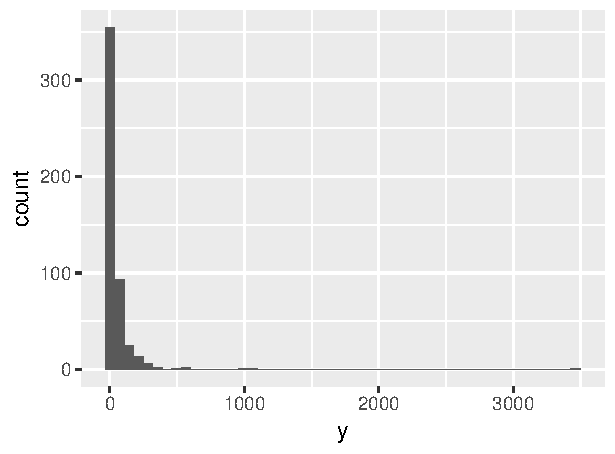
\includegraphics[width=0.45\linewidth]{prob_1_raw_x.pdf}
    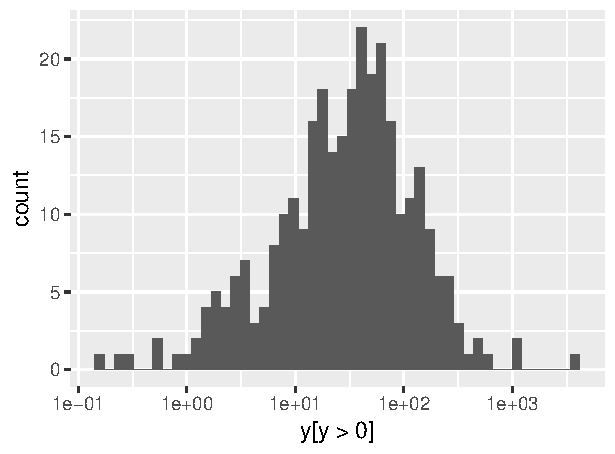
\includegraphics[width=0.45\linewidth]{prob_1_x_gr_0.pdf}
\end{figure}


We now use \texttt{stan} to do the computational inference. 

\subquestionwithpoints{3} To do so, we need to derive the target objective which is the log kernel of the posterior. Find it below:

\iftoggle{solutions}{\inred{
\beqn
&& \natlog{k(\bbeta, \theta_3, \theta_2~|~\X, \y)} \\
&=& \natlog{\theta_3^{n_0} (1 - \theta_3)^{n_+} \theta_2^{n_+} e^{-\parens{\displaystyle \sum_{~i : y_i > 0~} \x_i }\bbeta} \parens{\prod_{~i : y_i > 0~} 1 + y_i e^{-{\x_i\bbeta}}}^{-(\theta_2 + 1)}} \\
&=& n_0 \natlog{\theta_3} + n_+ \natlog{1 - \theta_3} + n_+ \natlog{\theta_2} - \parens{ \sum_{~i : y_i > 0~} \x_i }\bbeta -(\theta_2 + 1) \sum_{~i : y_i > 0~} \natlog{1 + y_i e^{-{\x_i\bbeta}}}
\eeqn
}}{~\spc{3}}
\pagebreak


We now do 5,000 samples in \texttt{stan}. Below is a histogram of the samples for $\theta_3$ produced by our visualize chains functions we used in class:

\begin{figure}[h]
    \centering
    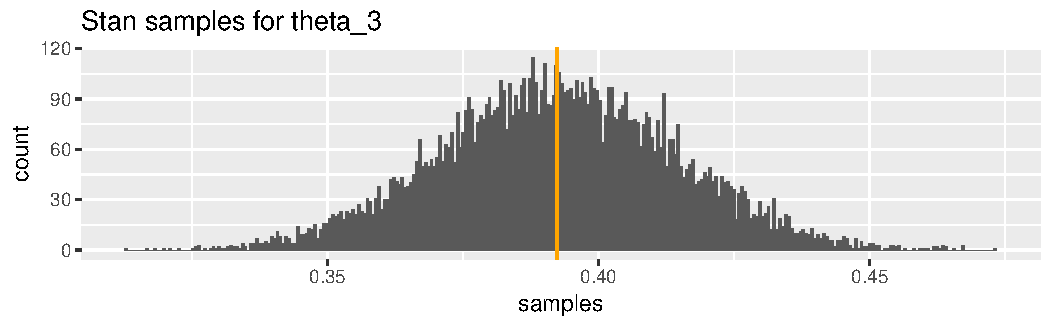
\includegraphics[width=1\linewidth]{theta3s.pdf}
\end{figure}


\subquestionwithpoints{3} Find a 95\% credible region for $\theta_3$.

\iftoggle{solutions}{\inred{
$CR_{\theta_3, 95\%} = \bracks{0.35, 0.44}$
}}{~\spc{1}}


Below is a histogram of the samples for $\theta_2$ produced by our visualize chains functions we used in class:

\begin{figure}[h]
    \centering
    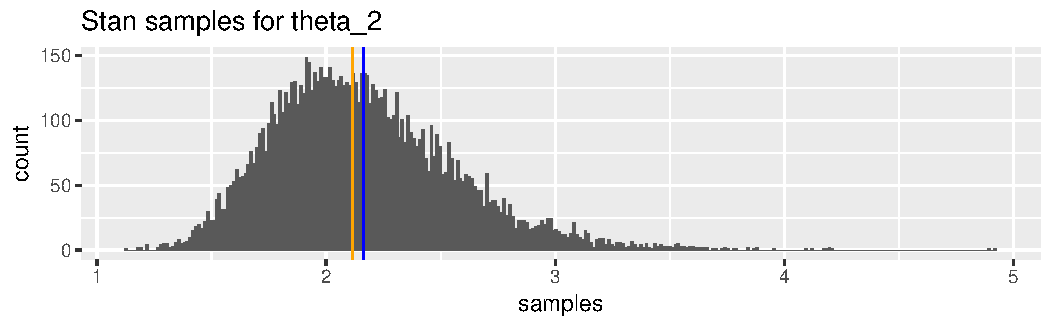
\includegraphics[width=1\linewidth]{theta2s.pdf}
\end{figure}

\subquestionwithpoints{4} The Lomax is a very interesting distribution. If $\theta_2 < 2$, the distribution has infinite or undefined variance (see problem header). Given the data we've seen, what is the probability our DGP has infinite or undefined variance assuming this model?

\iftoggle{solutions}{\inred{
$\cprob{\theta_2 < 2}{\X,\y} \approx 40\%$.
}}{~\spc{1}}

\pagebreak

Below are histograms of the samples for all $\beta_j$'s produced by our visualize chains functions we used in class:

\begin{figure}[h]
    \centering
    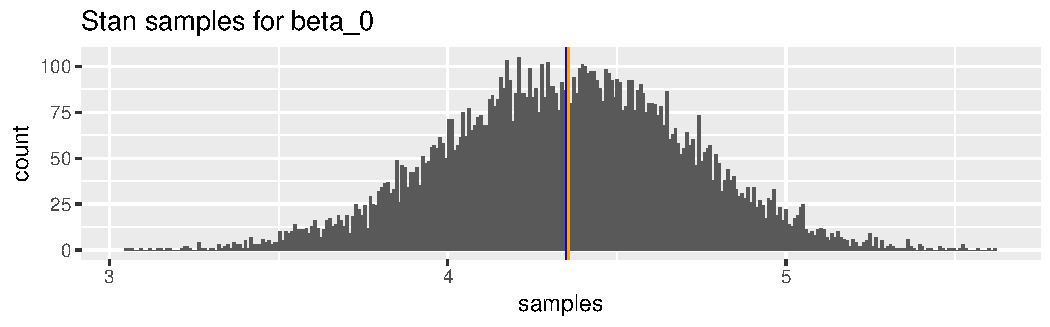
\includegraphics[width=0.8\linewidth]{beta0s.pdf}
    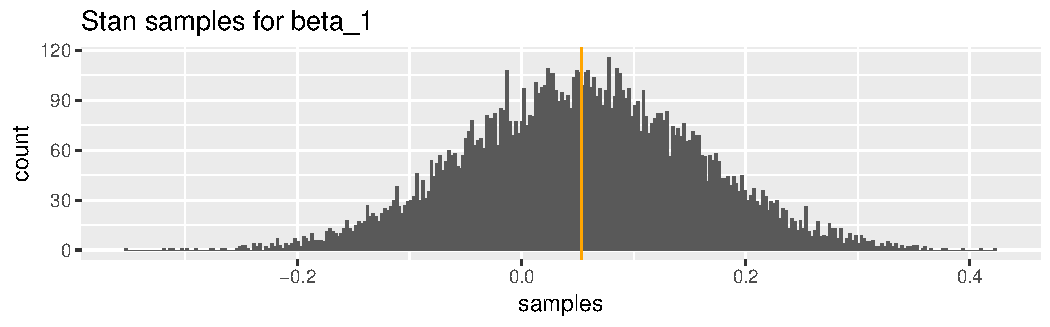
\includegraphics[width=0.8\linewidth]{beta1s.pdf}
    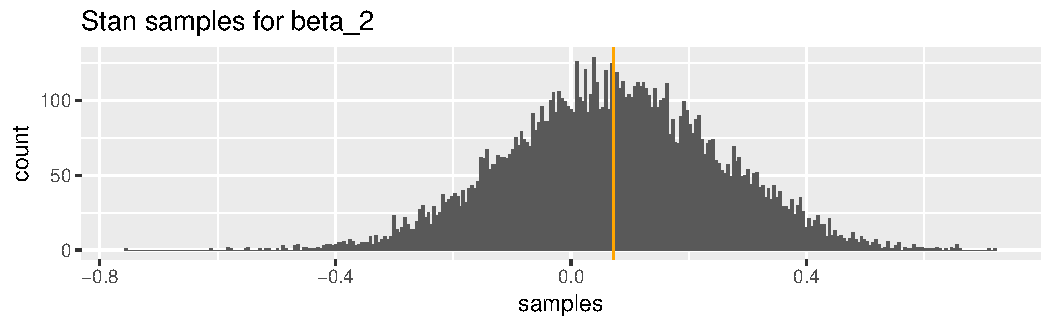
\includegraphics[width=0.8\linewidth]{beta2s.pdf}
    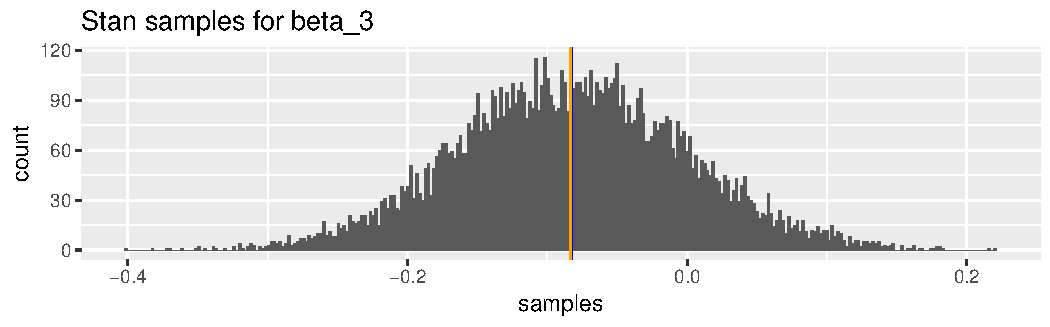
\includegraphics[width=0.8\linewidth]{beta3s.pdf}
\end{figure}
\vspace{-0.5cm}

\subquestionwithpoints{5} Make a decision about the omnibus test (i.e., the null hypothesis is that none of the three features matter in the linear model). Justify your decision.

\iftoggle{solutions}{\inred{
Since (a) $H_0: \beta_1 = 0$, $H_0: \beta_2 = 0$ and $H_0: \beta_3 = 0$ will be retained at any reasonable $\delta$ or (b) CR's for $\beta_1, \beta_2, \beta_3$ will all include zero at any reasonable $\alpha$, we can assume that we must also retain the omnibus null hypothesis that $H_0: \beta_1 = \beta_2 = \beta_3 = 0$.
}}{~\spc{1}}

\pagebreak

Regardless of what you answered in (h), you now want to examine the following company where $\x_\star = \bracks{2~1~5}$ as they have 2 cofounders, it's a tech company and they raised \$5M in their seed round. 

\subquestionwithpoints{3} Estimate the probability this company will fail (i.e., return zero).

\iftoggle{solutions}{\inred{
This is our best guess of $\theta_3$, the hurdle probability which is unaffected by $\x$. See top illustration on previous page for the MCMC samples. The best guess of $\theta_3$ given by the vertical line which is both the average value and median value is $\approx 39\%$.
}}{~\spc{1}}

\subquestionwithpoints{5} Assuming this company does not fail, what is the prediction of their return multiple, $y_\star$ rounded to two decimals?

\iftoggle{solutions}{\inred{
This is the expectation of the Lomax whose formula is given in the problem header. We need the link function, all the $\beta_j$ estimates and $\theta_2$:

\beqn
y_\star = \expe{Y~|~\x_\star} = \frac{\theta_{1,\star}}{\theta_2 - 1} =  \frac{e^{\x_\star \b}}{\theta_2 - 1} = \frac{e^{b_0 + b_1 x_1 + b_2 x_2 + b_3 x_3}}{\theta_2 - 1} \\
= \frac{\exp{4.3 + 0.05(2) + 0.1 (1) + -0.1 (5)}}{2.1 - 1} = 49.63
\eeqn
}}{~\spc{5}}

\end{enumerate}


\problem Consider a design matrix $\X$ of size $n \times (p+1)$ whose first column is $\onevec_n$ and whose rows are real measurements corresponding to response values in the vector $\y \in \reals^n$. We have reason to believe most of these features are uninformative to the response. We use the following algorithms to generate linear coefficients:

\beqn
\mathcal{A}_1:~\b_{\mathcal{A}_1} &=& \argmin_{\w \in \reals^{p+1}}\braces{(\y - \X\w)^\top (\y - \X\w)} \\
\mathcal{A}_2:~\b_{\mathcal{A}_2} &=& \argmin_{\w \in \reals^{p+1}}\braces{(\y - \X\w)^\top (\y - \X\w) + \lambda \sum_{j=1}^p w_j^2} ~~\text{where}~~ \lambda > 0\\
\mathcal{A}_3:~\b_{\mathcal{A}_3} &=& \argmin_{\w \in \reals^{p+1}}\braces{(\y - \X\w)^\top (\y - \X\w) + \gamma \sum_{j=1}^p |w_j|} ~~\text{where}~~ \gamma > 0
\eeqn


\begin{enumerate}[(a)]

\subquestionwithpoints{3} What are the names of these three algorithms?

\iftoggle{solutions}{\inred{
$\mathcal{A}_1:$ OLS \\
$\mathcal{A}_2:$ Ridge regression \\
$\mathcal{A}_3:$ Lasso regression
}}{~\\
$\mathcal{A}_1:$ \\~\\
$\mathcal{A}_2:$ \\~\\
$\mathcal{A}_3:$ 
}
\pagebreak

\subquestionwithpoints{2} For algorithms $\mathcal{A}_2$ and $\mathcal{A}_3$, what is a recommended prestep to do before running the algorithms?

\iftoggle{solutions}{\inred{
Standardizing the values in columns 2, \ldots, $p+1$ to have average zero and standard deviation one.
}}{~\spc{2}}

% \subquestionwithpoints{6} Assume the necessary prestep was executed and all fits are computed. Fill in the blanks in following terms using one of the following symbols $>,<,\geq,\leq,=,?$ where \qu{?} should be used only if the comparison is not possible. Express the relationships that are expected (those that we spent time studying in class).\\

% $||\b_{\mathcal{A}_1}||$  \iftoggle{solutions}{\inred{$<$}}{~\line(1,0){15}~} $||\b_{\mathcal{A}_2}||$,~~~~~~~~~
% $||\b_{\mathcal{A}_1}||$ \iftoggle{solutions}{\inred{$<$}}{~\line(1,0){15}~}     $||\b_{\mathcal{A}_3}||$,~~~~~~~~~
% $||\b_{\mathcal{A}_2}||$ \iftoggle{solutions}{\inred{$?$}}{~\line(1,0){15}~}      $||\b_{\mathcal{A}_3}||$


\subquestionwithpoints{5} Circle all the following statements that are true.

\begin{itemize}
    \item \iftoggle{solutions}{\inred{TRUE}}{} If $\lambda = 0,~~ ||\b_{\mathcal{A}_1}|| = ||\b_{\mathcal{A}_2}||$
    \item $\exists \lambda > 0,~~ ||\b_{\mathcal{A}_1}|| = ||\b_{\mathcal{A}_2}||$
    \item $\exists \gamma > 0,~~ ||\b_{\mathcal{A}_1}|| = ||\b_{\mathcal{A}_3}||$
    \item \iftoggle{solutions}{\inred{TRUE}}{} $\exists \lambda > 0, \gamma > 0,~~ ||\b_{\mathcal{A}_2}|| = ||\b_{\mathcal{A}_3}||$
    \item \iftoggle{solutions}{\inred{TRUE}}{} $\displaystyle\lim_{\lambda \rightarrow \infty} ||\b_{\mathcal{A}_2}|| = 0$
\end{itemize}


\subquestionwithpoints{3} Below are three columns each a sample of entries in $\b$ for some of the $p$ features. Match the most likely algorithms (1, 2, 3) to each of the columns by filling in the lines below the columns with a permutation of $\mathcal{A}_1, \mathcal{A}_2, \mathcal{A}_3$.

\begin{verbatim}
0.000000   -0.3600379  -0.2044754
0.000000   -0.0497710  -0.1043836
0.000000    2.2921732   3.7036262
0.000000   -0.0756272  -0.4866566
0.000000   -5.7274435  -7.4075626
2.866342    3.1096124   3.1156581
0.000000    0.3457908   0.2125626
0.000000   -3.1055237  -3.5124361
0.000000    3.7399084   5.4601868
0.000000   -2.6364656  -4.6368675
-1.352798  -3.6628336  -4.6743968
0.1619854  -0.1791046  -0.1105668
-3.440234  -4.5821048  -4.0857243
0.0000000   0.2331904   0.6371670
0.0000000  -0.1589228  -0.4134656
0.0000000   0.5340268   0.6212814
0.0000000  -0.2324948  -0.4902040
0.0000000   0.1720569   0.3553368
0.0000000  -1.7887053  -2.1417532
0.0000000   0.2537185   0.0777026
\end{verbatim}

\iftoggle{solutions}{\inred{$\mathcal{A}_3$~~~~~~~~~~~~~~}}{~\line(1,0){40}~~~~~~~~}
\iftoggle{solutions}{\inred{$\mathcal{A}_2$~~~~~~~~~~~~~~}}{\line(1,0){40}~~~~~~~~}
\iftoggle{solutions}{\inred{$\mathcal{A}_1$}}{\line(1,0){40}~}


\end{enumerate}
\pagebreak

\problem For each of the following, you will be provided with a DAG that includes observed metrics $x_1, x_2$ and an observed response $y$. These DAGs should be considered complete and self-contained, i.e. there are no other variables in the system and thus no noise. You will then be shown a series of predictive models with with OLS on a simple random sample of data points $\angbraces{x_{1,1}, x_{2,1}, y_1}, \ldots, \angbraces{x_{1,n}, x_{2,n}, y_n}$. 

For each problem, circle all coefficient estimates that are \textit{unbiased} estimates of the \textit{causal} effect of $x_1$ on $y$ (and/or $x_2$ on $y$). Note: a causal estimand of zero is still a real estimand. Here is an example done for you:

\begin{figure}[h]
    \centering
    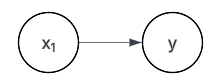
\includegraphics[width=0.3\linewidth]{causal0.png}\\
    
    $\hat{y} = b_0 + \Circled{\,b_1\,} x_1$
\end{figure}

\begin{enumerate}[(a)]


\subquestionwithpoints{4} 
\begin{figure}[h]
    \centering
    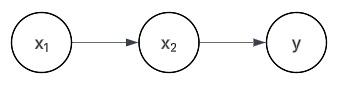
\includegraphics[width=0.5\linewidth]{causal2.png}
\end{figure}

\beqn
\hat{y} &=& b_0 + \iftoggle{solutions}{\inred{b_1}}{b_1} x_1 \\
\hat{y} &=& b_0 +           \iftoggle{solutions}{\inred{b_2}}{b_2} x_2\\
\hat{y} &=& b_0 + b_1 x_1 + \iftoggle{solutions}{\inred{b_2}}{b_2} x_2
\eeqn

\subquestionwithpoints{4} 
\begin{figure}[h]
    \centering
    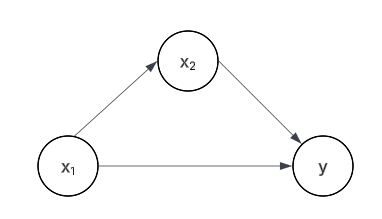
\includegraphics[width=0.5\linewidth]{causal1.png}
\end{figure}

\beqn
\hat{y} &=& b_0 + \iftoggle{solutions}{\inred{b_1}}{b_1} x_1 \\
\hat{y} &=& b_0 +           b_2 x_2\\
\hat{y} &=& b_0 + b_1 x_1 + \iftoggle{solutions}{\inred{b_2}}{b_2} x_2
\eeqn
\pagebreak

\subquestionwithpoints{1} 
\begin{figure}[h]
    \centering
    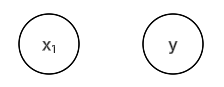
\includegraphics[width=0.3\linewidth]{causal00.png}
\end{figure}

\beqn
\hat{y} &=& b_0 + \iftoggle{solutions}{\inred{b_1}}{b_1} x_1
\eeqn

\subquestionwithpoints{4} 
\begin{figure}[h]
    \centering
    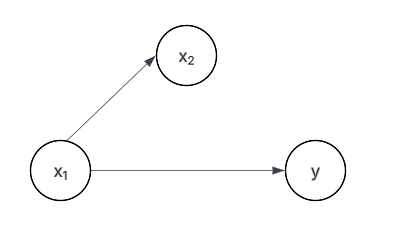
\includegraphics[width=0.5\linewidth]{causal4.png}
\end{figure}

\vspace{-0.5cm}
\beqn
\hat{y} &=& b_0 + \iftoggle{solutions}{\inred{b_1}}{b_1} x_1 \\
\hat{y} &=& b_0 +           b_2 x_2\\
\hat{y} &=& b_0 + \iftoggle{solutions}{\inred{b_1}}{b_1} x_1 + \iftoggle{solutions}{\inred{b_2}}{b_2} x_2
\eeqn


\subquestionwithpoints{4} 
\begin{figure}[h]
    \centering
    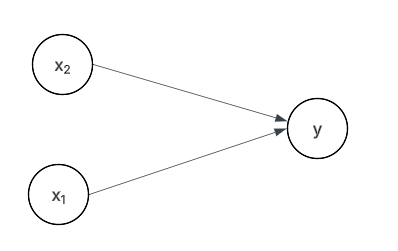
\includegraphics[width=0.5\linewidth]{causal3.png}
\end{figure}

\vspace{-0.5cm}
\beqn
\hat{y} &=& b_0 + \iftoggle{solutions}{\inred{b_1}}{b_1} x_1 \\
\hat{y} &=& b_0 +           \iftoggle{solutions}{\inred{b_2}}{b_2} x_2\\
\hat{y} &=& b_0 + \iftoggle{solutions}{\inred{b_1}}{b_1} x_1 + \iftoggle{solutions}{\inred{b_2}}{b_2} x_2
\eeqn
\pagebreak

\end{enumerate}


\problem The following questions are on experimental design. Let each of the rows be a subject in an experiment the $\x_{\cdot 1}$ column be the only covariate observed before the experiment begins. For each question, create two \textit{different} allocations $\w_1, \w_2$ from the \line(1,0){40} design for this experiment.

\begin{enumerate}[(a)]

\subquestionwithpoints{2} CRD \iftoggle{solutions}{\inred{
Any binary vectors will be correct here.
}}

\begin{table}[h]
    \centering
    \begin{tabular}{c||c|c}
        $\x_{\cdot 1}$ & ~~$\w_1$~~ & ~~$\w_2$~~  \\ \hline
        0.03 &&\\
        -0.74 &&\\
        0.19 &&\\
        -1.80 &&\\
        1.47  &&\\
        0.15  &&\\
        2.17 &&\\
        0.48  &&\\
    \end{tabular}
\end{table}



\vspace{-0.8cm}
\subquestionwithpoints{4} BCRD \iftoggle{solutions}{\inred{
As long as there are four zeroes and four ones in both columns, it will be correct.
}}

\begin{table}[h]
    \centering
    \begin{tabular}{c||c|c}
        $\x_{\cdot 1}$ & ~~$\w_1$~~ & ~~$\w_2$~~  \\ \hline
        0.03 &&\\
        -0.74 &&\\
        0.19 &&\\
        -1.80 &&\\
        1.47  &&\\
        0.15  &&\\
        2.17 &&\\
        0.48  &&\\
    \end{tabular}
\end{table}

\vspace{-0.3cm}
\subquestionwithpoints{6} blocking with $B=2$  \iftoggle{solutions}{\inred{
We have a continuous covariate so we sort it to obtain block \#1 of the smallest four values $-1.80, -0.74,  0.03,  0.15$, and block \#2 of the highest four values $0.19,  0.48,  1.47,  2.17$. The first block will be the subjects corresponding to the smallest four values and the second block to be the subjects corresponding to the highest four values. It is correct if there are two zeroes and two ones in each block.
}}

\begin{table}[h]
    \centering
    \begin{tabular}{c||c|c}
        $\x_{\cdot 1}$ & ~~$\w_1$~~ & ~~$\w_2$~~  \\ \hline
        0.03 &&\\
        -0.74 &&\\
        0.19 &&\\
        -1.80 &&\\
        1.47  &&\\
        0.15  &&\\
        2.17 &&\\
        0.48  &&\\
    \end{tabular}
\end{table}
 
\pagebreak

\subquestionwithpoints{6} pairwise matching \iftoggle{solutions}{\inred{
The sorted values are \\ $-1.80, -0.74,  0.03,  0.15, 0.19,  0.48,  1.47,  2.17$ so the first pair consist of the subjects that have the covariates measurements $-1.80, -0.74$, the second pair consists of the subjects that have the covariates measurements $0.03,  0.15$, etc. As long as there is one zero and one one in each pair, it is correct.
}}

\begin{table}[h]
    \centering
    \begin{tabular}{c||c|c}
        $\x_{\cdot 1}$ & ~~$\w_1$~~ & ~~$\w_2$~~  \\ \hline
        0.03 &&\\
        -0.74 &&\\
        0.19 &&\\
        -1.80 &&\\
        1.47  &&\\
        0.15  &&\\
        2.17 &&\\
        0.48  &&\\
    \end{tabular}
\end{table}

\end{enumerate}

\vspace{-0.5cm}
\problem The following questions are on based on glm's.


\begin{enumerate}[(a)]

\subquestionwithpoints{5} Consider the following code and snippet of its output:

\begin{Verbatim}[frame=single]
> pima = na.omit(MASS::Pima.tr2)
> pima$type = ifelse(pima$type == "Yes", 1, 0)
> summary(glm(type ~ ., pima, family = binomial(link = "logit")))

             Estimate Std. Error z value Pr(>|z|)    
(Intercept) -9.773062   1.770386  -5.520 3.38e-08 ***
npreg        0.103183   0.064694   1.595  0.11073    
glu          0.032117   0.006787   4.732 2.22e-06 ***
bp          -0.004768   0.018541  -0.257  0.79707    
\end{Verbatim}

Assume the data was collected using a simple random sample of subjects and that the \texttt{type} being equal to \qu{\texttt{Yes}} means the subject has diabetes otherwise not. Provide an interpretation of the estimated coefficient of \texttt{glu} which is measured in mg/dL.

\iftoggle{solutions}{\inred{
When comparing two subjects (A) and (B) which are sampled in the same fashion as the other subjects in this dataset where (A) has a \texttt{glu} measurement 1mg/dL larger than (B)'s \texttt{glu} measurement but share the same other observed measurements otherwise, then (A) is predicted to have an estimated log odds probability of diabetes 0.032 $\pm$ 0.007 higher than (B)'s log odds probability of diabetes assuming the log odds probability of diabetes is linear in the measurements considered herein.
}}{~\spc{3}}
\pagebreak

\subquestionwithpoints{5} Consider the following code and snippet of its output:

\begin{Verbatim}[frame=single]
> lung = na.omit(survival::lung)
> lung$status = lung$status - 1 #needs to be 0=alive, 1=dead
> surv_obj = Surv(lung$time, lung$status)
> full_mod = survreg(surv_obj ~ . - time - status, lung)
> summary(full_mod)

                Value Std. Error     z       p
(Intercept)  7.17e+00   1.08e+00  6.64 3.2e-11
inst         2.05e-02   8.80e-03  2.32  0.0201
age         -7.54e-03   8.06e-03 -0.94  0.3497
sex          3.91e-01   1.39e-01  2.82  0.0048
ph.ecog     -6.26e-01   1.58e-01 -3.95 7.7e-05
ph.karno    -1.86e-02   7.67e-03 -2.43  0.0151
pat.karno    7.68e-03   5.54e-03  1.39  0.1656
meal.cal     7.32e-06   1.81e-04  0.04  0.9678
wt.loss      1.10e-02   5.34e-03  2.07  0.0387
Log(scale)  -3.76e-01   7.28e-02 -5.17 2.3e-07

Scale= 0.686 
\end{Verbatim}

Assume the data was collected using a simple random sample of subjects, and the variable \texttt{ph.ecog} (which is measured in \qu{score units}) was experimentally manipulated in the subjects while all other variables were observed naturally. The variable \texttt{time} is measured in units of days. Provide an interpretation of the estimated coefficient of \texttt{ph.ecog}.


\iftoggle{solutions}{\inred{
If \texttt{ph.ecog} is increased by one score unit and all other measurements remain constant, the [log survival of the subject in days will resultingly decrease by an estimated 0.626 $\pm$ 0.158] assuming subject survival-in-days is Weibull-distributed with log mean linear in the measurements considered herein. \\

You can alternatively replace the above bracketed text with \qu{the survival of the subject in days will resultingly decrease by 46.5\%} where that value is calculated as $1-e^{-0.626}$.
}}{~\spc{3}}
\pagebreak

\end{enumerate}



\problem This is the same setup as problem 1 from Midterm II. Consider the following full-rank design matrix:

\beqn
\X := \bracks{\onevec_n~|~\x_{\cdot 1}~|~\ldots~|~ \x_{\cdot p}} = \threevec{\x_{1 \cdot}}{\vdots}{\x_{n \cdot}}
\eeqn

\noindent with column indices $0, 1, \ldots, p$ and row indices $1, 2, \ldots, n$. Let $\H$ be the orthogonal projection matrix onto the column space of $\X$ and let $\I_n - \H$ be the orthogonal projection matrix onto the column space of $\X_\perp$. We assume also a continuous (real-valued) response model which is linear in these measurements, i.e. $\Y = \X\bbeta + \berrorrv$. For the error term, we assume the \qu{core assumption},

\beqn
\berrorrv \sim \multnormnot{n}{\zerovec_n}{\sigsq \I_n} ~~~\text{where $\sigsq>0$}.
\eeqn

\noindent Consider the following estimator for $\bbeta$: $\B := \XtXinvXt \Y$ and let $\Yhat := \X\B$ and $\E := \Y - \Yhat$.

\begin{enumerate}[(a)]

\subquestionwithpoints{5} Derive the distribution of $\E$ with only what is in the problem header, the fact about multivariate normal distributions from 340 and linear algebra manipulations. Show each step.

\iftoggle{solutions}{\inred{
\beqn
\E &=& (\I_n - \H) \Y \\
&=& (\I_n - \H) \parens{\X\bbeta + \berrorrv} \\
&=& (\I_n - \H)\X\bbeta + (\I_n - \H)\berrorrv\\ 
&=& (\I_n - \H)\berrorrv\\
&\sim& \multnormnot{n}{\zerovec_{n}}{(\I_n - \H) \sigsq \I_n (\I_n - \H)^\top} \\
&=& \multnormnot{n}{\zerovec_{n}}{\sigsq (\I_n - \H)}
\eeqn
}}{~\spc{5}}

\end{enumerate}

\end{document}


\pagebreak






\problem Consider the Boston Housing Data which has $n = 506$ and response \texttt{medv} with $\ybar = 22.53$ and $s_y = 9.20$. We consider modeling \texttt{medv} using OLS on \texttt{zn + rm + nox + dis + lstat}, all continuous (non-categorical) features. Below is the $\XtXinv$ where $\X$ is the design matrix:

\begin{Verbatim}[frame=single, fontsize = \small]
            (Intercept)       zn       rm      nox      dis    lstat
(Intercept)     0.58000  4.4e-04 -5.1e-02 -2.7e-01 -1.8e-02 -3.0e-03
zn              0.00044  6.9e-06 -4.5e-05 -7.1e-05 -5.1e-05 -2.0e-07
rm             -0.05100 -4.5e-05  6.9e-03  7.5e-04  6.3e-04  4.4e-04
nox            -0.27000 -7.1e-05  7.5e-04  4.2e-01  1.5e-02 -1.9e-03
dis            -0.01800 -5.1e-05  6.3e-04  1.5e-02  1.5e-03  4.3e-05
lstat          -0.00300 -2.0e-07  4.4e-04 -1.9e-03  4.3e-05  8.9e-05
\end{Verbatim}

\noindent The RMSE for this regression is 5.289 and here are the slope estimates:


\begin{Verbatim}[frame=single, fontsize = \small]
(Intercept)          zn          rm         nox         dis       lstat 
      16.14        0.06        4.44      -15.20       -1.44       -0.66
\end{Verbatim}

\noindent Assume the \qu{core assumption} (see Problem 1 for its definition) except in (e,f,l,m) which make explicit a new assumption.

\begin{enumerate}[(a)]

\subquestionwithpoints{2} Consider creating a $\doublehat{CI}_{\beta_{\texttt{nox}}, 95\%}$, the confidence interval for the true slope parameter of the variable \texttt{nox}. Which degrees of freedom value would you use to lookup the appropriate $t$ value's quantile? 

\iftoggle{solutions}{\inred{
\beqn
df_{\text{error}} := n-(p+1) = 506 - 6 = 500
\eeqn
}}{~\spc{0}}

\pagebreak


\subquestionwithpoints{5} Compute $\doublehat{CI}_{\beta_{\texttt{nox}}, 95\%}$ to the nearest two digits. Regardless of the truly appropriate $t$ value, use 1.96 as the $t$ value.

\iftoggle{solutions}{\inred{
\beqn
\doublehat{CI}_{\beta_{\texttt{nox}}, 1 - \alpha} &=& \bracks{b_{\texttt{nox}} \pm t_{df_{\text{error}}, 1 - \alpha/2} \cdot s_e \sqrt{\XtXinv_{\texttt{nox}, \texttt{nox}}}} \\
\doublehat{CI}_{\beta_3, 95\%} &=& \bracks{b_3 \pm 1.96 \cdot s_e \sqrt{\XtXinv_{4,4}}} \\
&=& \bracks{-15.20 \pm 1.96 \cdot 5.289 \sqrt{0.42}} = \bracks{-21.92,  -8.48}
\eeqn
}}{~\spc{3.5}}


\subquestionwithpoints{1} The confidence interval in the previous question is... circle one: \\\iftoggle{solutions}{\inred{exact}}{exact} ~~/~~ approximate

\subquestionwithpoints{1} Based on your confidence interval from the previous question, the null hypothesis that $\beta_{\texttt{nox}} = 0$ would be ... circle one: \\\iftoggle{solutions}{\inred{rejected}}{rejected} ~~/~~ retained

\subquestionwithpoints{5} Assume the errors are independent, mean centered and homoskedastic but now assume they are \textit{not} normally distributed. Create a $\doublehat{CI}_{\beta, 95\%}$ for the variable \texttt{nox} to the nearest two digits.

\iftoggle{solutions}{\inred{
\beqn
\bracks{-21.92,  -8.48}
\eeqn
}}{~\spc{1}}

\subquestionwithpoints{1} The confidence interval in the previous question is... circle one: \\ exact ~~/~~ \iftoggle{solutions}{\inred{approximate}}{approximate}


\subquestionwithpoints{5} Justify and record your decision for the test of $H_0: \beta_{\texttt{rm}} = 3$, a test on the slope parameter for the variable \texttt{rm}. Regardless of the truly appropriate $t$ value, use 1.96 as the $t$ value.

\iftoggle{solutions}{\inred{
\beqn
\doublehat{t} := \frac{b_{\texttt{rm}} - \beta_{\texttt{rm}}}{s_e \cdot \sqrt{\XtXinv_{\texttt{rm}, \texttt{rm}}}} = \frac{4.44 - 3}{5.289 \cdot \sqrt{0.0069}} = 3.277 > 1.96 \mathimplies \text{Reject $H_0$}
\eeqn
}}{~\spc{3}}

\pagebreak

\subquestionwithpoints{5} Compute $R^2_{adj}$ to the nearest two digits using the following calculations:

\beqn
s_e &:=& \sqrt{\frac{SSE}{df_{\text{error}}}} \mathimplies SSE = df_{\text{error}} \cdot s_e^2  = 500 \cdot 5.289^2   = 13986.76 \\
SST &:=& \sum_{i=1}^n (y_i - \ybar)^2 = (n-1) \cdot s^2_y = 505 \cdot 9.20^2  = 42743.2
\eeqn



\iftoggle{solutions}{\inred{
\beqn
R^2_{adj} &:=& 1 - \frac{n-1}{df_{\text{error}}} \frac{SSE}{SST} = \frac{505}{500} \frac{13986.76}{42743.2} = 0.33\\
\eeqn
}}{~\spc{3}}

Below is the first six rows and six columns of the $\H$ matrix. There are rownames and colnames displayed to help with finding entries (e.g., $\H_{2,4} = 0.0076$).

\begin{center}
\begin{minipage}{10cm}
\begin{Verbatim}[frame=single]
       1      2      3      4      5      6
1 0.0053 0.0020 0.0035 0.0039 0.0024 0.0036
2 0.0020 0.0058 0.0065 0.0076 0.0076 0.0072
3 0.0035 0.0065 0.0100 0.0110 0.0110 0.0085
4 0.0039 0.0076 0.0110 0.0130 0.0130 0.0110
5 0.0024 0.0076 0.0110 0.0130 0.0140 0.0110
6 0.0036 0.0072 0.0085 0.0110 0.0110 0.0110
\end{Verbatim}
\end{minipage}
\end{center}

\subquestionwithpoints{5} Estimate the probability the residual for the fourth observation in the boston housing dataset will be greater than 5 as best as you can.

\iftoggle{solutions}{\inred{
\beqn
&& E_4 \sim \normnot{0}{\sigsq (1 - h_{4,4})} \mathimplies \frac{E_4}{\sigma \sqrt{1 - h_{4,4}}} \sim \stdnormnot \mathimplies \frac{E_4}{s_e \sqrt{1 - h_{4,4}}} \approxdist \stdnormnot \\
&& \prob{E_4 > 5} = \prob{\frac{E_4}{s_e \sqrt{1 - h_{4,4}}} > \frac{5}{s_e \sqrt{1 - h_{4,4}}}} \approx \prob{Z > \frac{5}{5.289\sqrt{1 - 0.0130}}} \\
 &=& \prob{Z > 0.95} \approx 16\%
\eeqn
}}{~\spc{3}}

\pagebreak

\subquestionwithpoints{6} The predicted value for the first observation is $\hat{y}_1 = 29.15$. Find a $\doublehat{CI}_{y_1, 95\%}$ where $y_1$ is the response value for a new census tract with the same measurements as $\x_{1 \cdot}$ to the nearest two digits.  Regardless of the truly appropriate $t$ value, use 1.96 as the $t$ value.

\iftoggle{solutions}{\inred{
\beqn
\doublehat{CI}_{y_1, 95\%} &=& \bracks{\hat{y}_1 \pm t_{1-\alpha/2, n - (p+1)} \cdot s_e\sqrt{1 + \x_{1 \cdot}^\top \XtXinv \x_{1 \cdot}}} \\
&=& \bracks{\hat{y}_1 \pm t_{1-\alpha/2, n - (p+1)} \cdot s_e\sqrt{1 + h_{1,1}}} \\
&=& \bracks{29.15 \pm 1.96 \cdot 5.289 \sqrt{1 + 0.0053}} = \bracks{18.76, 39.54}
\eeqn
}}{~\spc{6}}

We now model \texttt{medv} using \texttt{rm + lstat} via an OLS. The RMSE for this regression is 5.540 and here are the slope estimates:

\begin{center}
\begin{minipage}{8cm}
\begin{Verbatim}[frame=single]
(Intercept)          rm       lstat 
      -1.36        5.09       -0.64
\end{Verbatim}
\end{minipage}
\end{center}


\subquestionwithpoints{7} Calculate the F-statistic for $H_0: \beta_{\texttt{zn}} = \beta_{\texttt{nox}} = \beta_{\texttt{dis}} = 0$ to the nearest two digits.

\iftoggle{solutions}{\inred{
\beqn
\doublehat{f} := \frac{\displaystyle \frac{SSE_A - SSE}{k}}{\displaystyle\frac{SSE}{df_{error}}} = \frac{\displaystyle\frac{15437.87 - 13986.76}{3}}{\displaystyle\frac{13986.76}{500}} = 17.29
\eeqn

The value of $k$ is the number of features we are setting to zero in $H_0$ which is 3. The value of SSE we take from part (h). To obtain the value of $SSE_A$, see the calculation in part (h). $SSE_A = df_A s^2_{e_A}$ where the quantities on the rhs are now applicable to the reduced model with features in set $A$. Following part (a), $df_A = n - ((p-k) + 1) = 506 - ((5-3) + 1) = 503$. And $s^2_{e_A}$ can be found in the text above this question. Thus, $SSE_A = 503 \cdot 5.54^2 = 15437.87$. 
}}{~\spc{6}}


\pagebreak

Below is $\XtXinvXt \bv{\doublehat{D}} \X \XtXinv$, a matrix where $\X$ is the design matrix and $\bv{\doublehat{D}}$ is the diagonal matrix with the residuals squared along its diagonal.

\begin{center}
\begin{minipage}{8cm}
\begin{Verbatim}[frame=single]
            (Intercept)    rm lstat
(Intercept)       29.20 -4.14 -0.26
rm                -4.14  0.59  0.03
lstat             -0.26  0.03  0.00
\end{Verbatim}
\end{minipage}
\end{center}

\subquestionwithpoints{5} Assume the errors are independent, mean centered but neither homoskedastic nor normally distributed. Create a $\doublehat{CI}_{\beta_{\texttt{rm}}, 95\%}$, the confidence interval for the true slope parameter of the variable \texttt{rm} to the nearest two digits.

\iftoggle{solutions}{\inred{
\beqn
\doublehat{CI}_{\beta_{\texttt{rm}}, 1-\alpha} &=& \bracks{b_{\texttt{rm}} \pm z_{1-\alpha/2} \sqrt{\parens{\XtXinvXt \bv{\doublehat{D}} \X \XtXinv}_{\texttt{rm}, \texttt{rm}}}~} \\
\doublehat{CI}_{\beta_1, 95\%} &=& \bracks{b_1 \pm 1.96   \sqrt{\parens{\XtXinvXt \bv{\doublehat{D}} \X \XtXinv}_{2,2}}~} \\
&=& \bracks{5.09 \pm 1.96  \sqrt{0.59}} = \bracks{3.58, 6.60}
\eeqn
}}{~\spc{4}}

\subquestionwithpoints{1} The confidence interval in the previous question is... circle one: \\ exact ~~/~~ \iftoggle{solutions}{\inred{approximate}}{approximate}

\end{enumerate}


\problem Consider a subset of the vocab data in the \texttt{carData} package. The response is a person's score on a vocabulary test. This score ranges in $\braces{0, 1, 2, \ldots, 10}$ and features: \texttt{gender} (categorical: male/female), \texttt{nativeBorn} (categorical: yes/no), \texttt{age} (continuous: measured in years) and \texttt{educ} (continuous: measured in years). We will use a negative binomial glm with the standard exponential link-to-linear function for its mean. Below is the output:

\begin{center}
\begin{minipage}{13cm}
\begin{Verbatim}[frame=single]
               Estimate   Std. Error z value Pr(>|z|)    
(Intercept)    0.7761238  0.0165403  46.923  < 2e-16 ***
gendermale    -0.0267524  0.0049960  -5.355 8.57e-08 ***
nativeBornyes  0.1603976  0.0094713  16.935  < 2e-16 ***
age            0.0021438  0.0001438  14.907  < 2e-16 ***
educ           0.0582323  0.0008373  69.548  < 2e-16 ***

              Theta:  172454 
          Std. Err.:  143423

 2 x log-likelihood:  -115304.3 
\end{Verbatim}
\end{minipage}
\end{center}


\pagebreak

\begin{enumerate}[(a)]


\subquestionwithpoints{5} Is there any reason why we should not model this response metric using the negative binomial model with mean log-linear in the covariates?

\iftoggle{solutions}{\inred{
The response metric doesn't have the support of a true count model as it only ranges from $0,1,\ldots,10$ instead of the whole space $0, 1, \ldots$ and this means the model may give nonsensical predictions (i.e., vocabulary scores $>$ 10). Thus, the inference will also be suspect.
}}{~\spc{3}}

Despite what you wrote in (a), we will ignore any concerns about the appropriateness of this model going forward.

\subquestionwithpoints{5} Considering all other covariate values the same, what would be the predicted \textit{percent} difference in mean score of a male versus a female to the nearest two digits? 

\iftoggle{solutions}{\inred{
Since $\hat{y} = e^{b_0} e^{b_1 x_1} \cdot \ldots \cdot e^{b_p x_p}$, the prediction is affected by not an addition, but a multiple, $e^{b_j x_j}$, thus the percent effect is $(e^{b_j x_j} - 1) \times 100$. For the male-vs-female coefficient, we then get 

\beqn
(e^{-0.0267524} - 1) \times 100 = -2.64\%
\eeqn
}}{~\spc{3}}

\subquestionwithpoints{6} Compute $\doublehat{CI}_{\beta_{\texttt{educ}}, 95\%}$, the confidence interval for the slope parameter within the link function for the variable \texttt{educ} to the nearest four digits.

\iftoggle{solutions}{\inred{
\beqn
\doublehat{CI}_{\beta_{\texttt{educ}}, 1-\alpha} &=& \bracks{b_{\texttt{educ}} \pm z_{1-\alpha/2} \cdot s_{b_{\texttt{educ}}}} \\
\doublehat{CI}_{\beta_4, 95\%} &=& \bracks{b_4 \pm 1.96 \cdot s_{b_4}} \\
 &=& \bracks{0.0582323 \pm 1.96 \cdot 0.0008373} = \bracks{0.0566,  0.0599}
\eeqn
}}{~\spc{6}}


\subquestionwithpoints{1} The confidence interval in the previous question is... circle one: \\ exact ~~/~~ \iftoggle{solutions}{\inred{approximate}}{approximate}


\pagebreak

\subquestionwithpoints{6} Predict the vocabulary score of a female, foreign-born, age 25 with 17yr of education. Round the score to the nearest whole number.

\iftoggle{solutions}{\inred{
\beqn
\hat{y} &=& \text{round}\parens{e^{b_0} e^{b_1 x_1} \cdot \ldots \cdot e^{b_p x_p}} \\
&=& \text{round}\parens{e^{b_0} e^{b_1 (0)} e^{b_2 (0)} e^{b_3 (25)} e^{b_4 (17)}} \\
&=& \text{round}\parens{e^{0.7761238} e^{0.0021438 (25)} e^{0.0582323 (17)}} \\
&=& \text{round}(6.169809) = 6
\eeqn
}}{~\spc{6}}

We now run the same model but this time omitting features \texttt{gender} and \texttt{nativeBorn}. Below is the output


\begin{center}
\begin{minipage}{13cm}
\begin{Verbatim}[frame=single]
            Estimate   Std. Error  z value Pr(>|z|)    
(Intercept) 0.9130409  0.0139108   65.64   <2e-16 ***
age         0.0022436  0.0001438   15.61   <2e-16 ***
educ        0.0578375  0.0008323   69.49   <2e-16 ***

              Theta:  173175 
          Std. Err.:  146404

 2 x log-likelihood:  -115635.4
\end{Verbatim}
\end{minipage}
\end{center}

Here are some values of the inverse CDF of the $\chisq{df}$ distribution:

\begin{center}
\begin{minipage}{13cm}
\begin{Verbatim}[frame=single,fontsize=\small]
                Probability less than the critical value
  df          0.90      0.95     0.975      0.99     0.999
----------------------------------------------------------
  1          2.706     3.841     5.024     6.635    10.828
  2          4.605     5.991     7.378     9.210    13.816
  3          6.251     7.815     9.348    11.345    16.266
  4          7.779     9.488    11.143    13.277    18.467
  5          9.236    11.070    12.833    15.086    20.515
  6         10.645    12.592    14.449    16.812    22.458
  7         12.017    14.067    16.013    18.475    24.322
\end{Verbatim}
\end{minipage}
\end{center}

\pagebreak

\subquestionwithpoints{2} For the test of $H_0: \beta_{\texttt{gender}} = \beta_{\texttt{nativeBorn}} = 0$ at $\alpha = 1\%$, would would be the critical value of the likelihood ratio test that the test statistic is compared to?

\iftoggle{solutions}{\inred{
The degrees of freedom of this test is 2 because we are knocking out 2 features. Since $\alpha = 1\%$, we are looking for the 99\%ile of the $\chisq{2}$ which according we find in the table above on the second row and the fourth column: 9.210.
}}{~\spc{1}}

\subquestionwithpoints{7} Run the test of $H_0: \beta_{\texttt{gender}} = \beta_{\texttt{nativeBorn}} = 0$ at $\alpha = 1\%$ and record your decision and write one sentence that interprets the result of the decision.

\iftoggle{solutions}{\inred{
Since $\doublehat{\Lambda} = 2\natlog{\mathcal{L}_{\text{full}}} - 2\natlog{\mathcal{L}_{\text{reduced}}} = -115304.3 - -115635.4 = 331.1 > \chisq{2, 99\%} = 9.210$, we reject $H_0$. We can conclude that \texttt{gender} and \texttt{nativeBorn} are important in predicting vocabulary score in the context of the other variables and assuming the negative binomial model log-linear in the covariates.
}}{~\spc{7}}



\end{enumerate}

\end{document}
